\iffalse
\documentclass[10pt]{article}
\usepackage{graphicx}
\usepackage[none]{hyphenat}
\usepackage{graphicx}
\usepackage{listings}
\usepackage[english]{babel}
\usepackage{siunitx}
\usepackage{graphicx}
\usepackage{caption} 
\usepackage{booktabs}
\usepackage{array}
\usepackage{amssymb} % for \because
\usepackage{amsmath}   % for having text in math mode
\usepackage{extarrows} % for Row operations arrows
\usepackage{listings}
\usepackage[utf8]{inputenc}
\lstset{
  frame=single,
  breaklines=true
}
\usepackage{hyperref}
  
%Following 2 lines were added to remove the blank page at the beginning
\usepackage{atbegshi}% http://ctan.org/pkg/atbegshi
\AtBeginDocument{\AtBeginShipoutNext{\AtBeginShipoutDiscard}}


%New macro definitions
\newcommand{\mydet}[1]{\ensuremath{\begin{vmatrix}#1\end{vmatrix}}}
\providecommand{\brak}[1]{\ensuremath{\left(#1\right)}}
\newcommand{\solution}{\noindent \textbf{Solution: }}
\newcommand{\myvec}[1]{\ensuremath{\begin{pmatrix}#1\end{pmatrix}}}
\providecommand{\norm}[1]{\left\lVert#1\right\rVert}
\providecommand{\abs}[1]{\left\vert#1\right\vert}
\let\vec\mathbf{}
\begin{document}

\begin{center}
\title{\textbf{Three Dimensional Geometry}}
\date{\vspace{-5ex}} %Not to print date automatically
\maketitle
\end{center}
\section{12$^{th}$ Maths - Chapter 11}
This is Problem 5 from Exercise-11.2
\begin{enumerate}
\item Find the equation of the line in vector and in cartesian form that passes through the point with position vector $2\hat{i}-\hat{j}+4\hat{k}$ and is in direction $\hat{i}+2\hat{j}-\hat{k}$.

\solution
\fi
Let
\begin{align}
\vec{A}=\myvec{2\\-1\\4},\,\vec{m}=\myvec{1\\2\\-1}
\end{align}
Vector equation of a line is,
\begin{align}
\vec{x}=\vec{A}+\lambda\vec{m}
=\myvec{2\\-1\\4}+\lambda\myvec{1\\2\\-1}
\end{align}
See Fig. 
\ref{fig:chapters/12/11/2/5/Fig1}.
\begin{figure}[h!]
	\begin{center}
		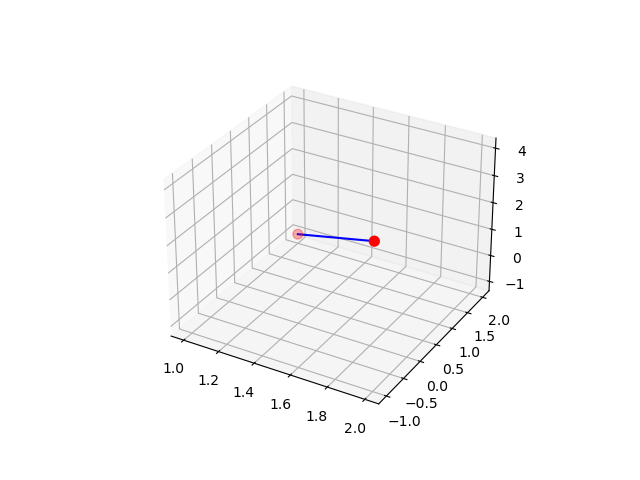
\includegraphics[width=\columnwidth]{./chapters/12/11/2/5/figs/fig.png}
	\end{center}
\caption{}
\label{fig:chapters/12/11/2/5/Fig1}
\end{figure}
